\documentclass{standalone}
\usepackage{tikz}
\usetikzlibrary{positioning,arrows.meta,shapes.misc,calc}

% COLORS
\usepackage{xcolor}
\colorlet{myred}{red!80!black}
\colorlet{myblue}{blue!80!black}
\colorlet{mybluee}{myblue!80!black}
\colorlet{mygreen}{green!60!black}
\colorlet{myorange}{orange!70!red!60!black}
\colorlet{mydarkred}{red!30!black}
\colorlet{mydarkblue}{blue!40!black}
\colorlet{mydarkgreen}{green!30!black}
\definecolor{mygray}{HTML}{D1D2D4}

\begin{document}
\begin{tikzpicture}[
    >=Stealth,
    block/.style={rectangle, rounded corners, draw, align=center},
]

% Placeholder image
\node[inner sep=0, outer sep=0] (image) at (0,0) {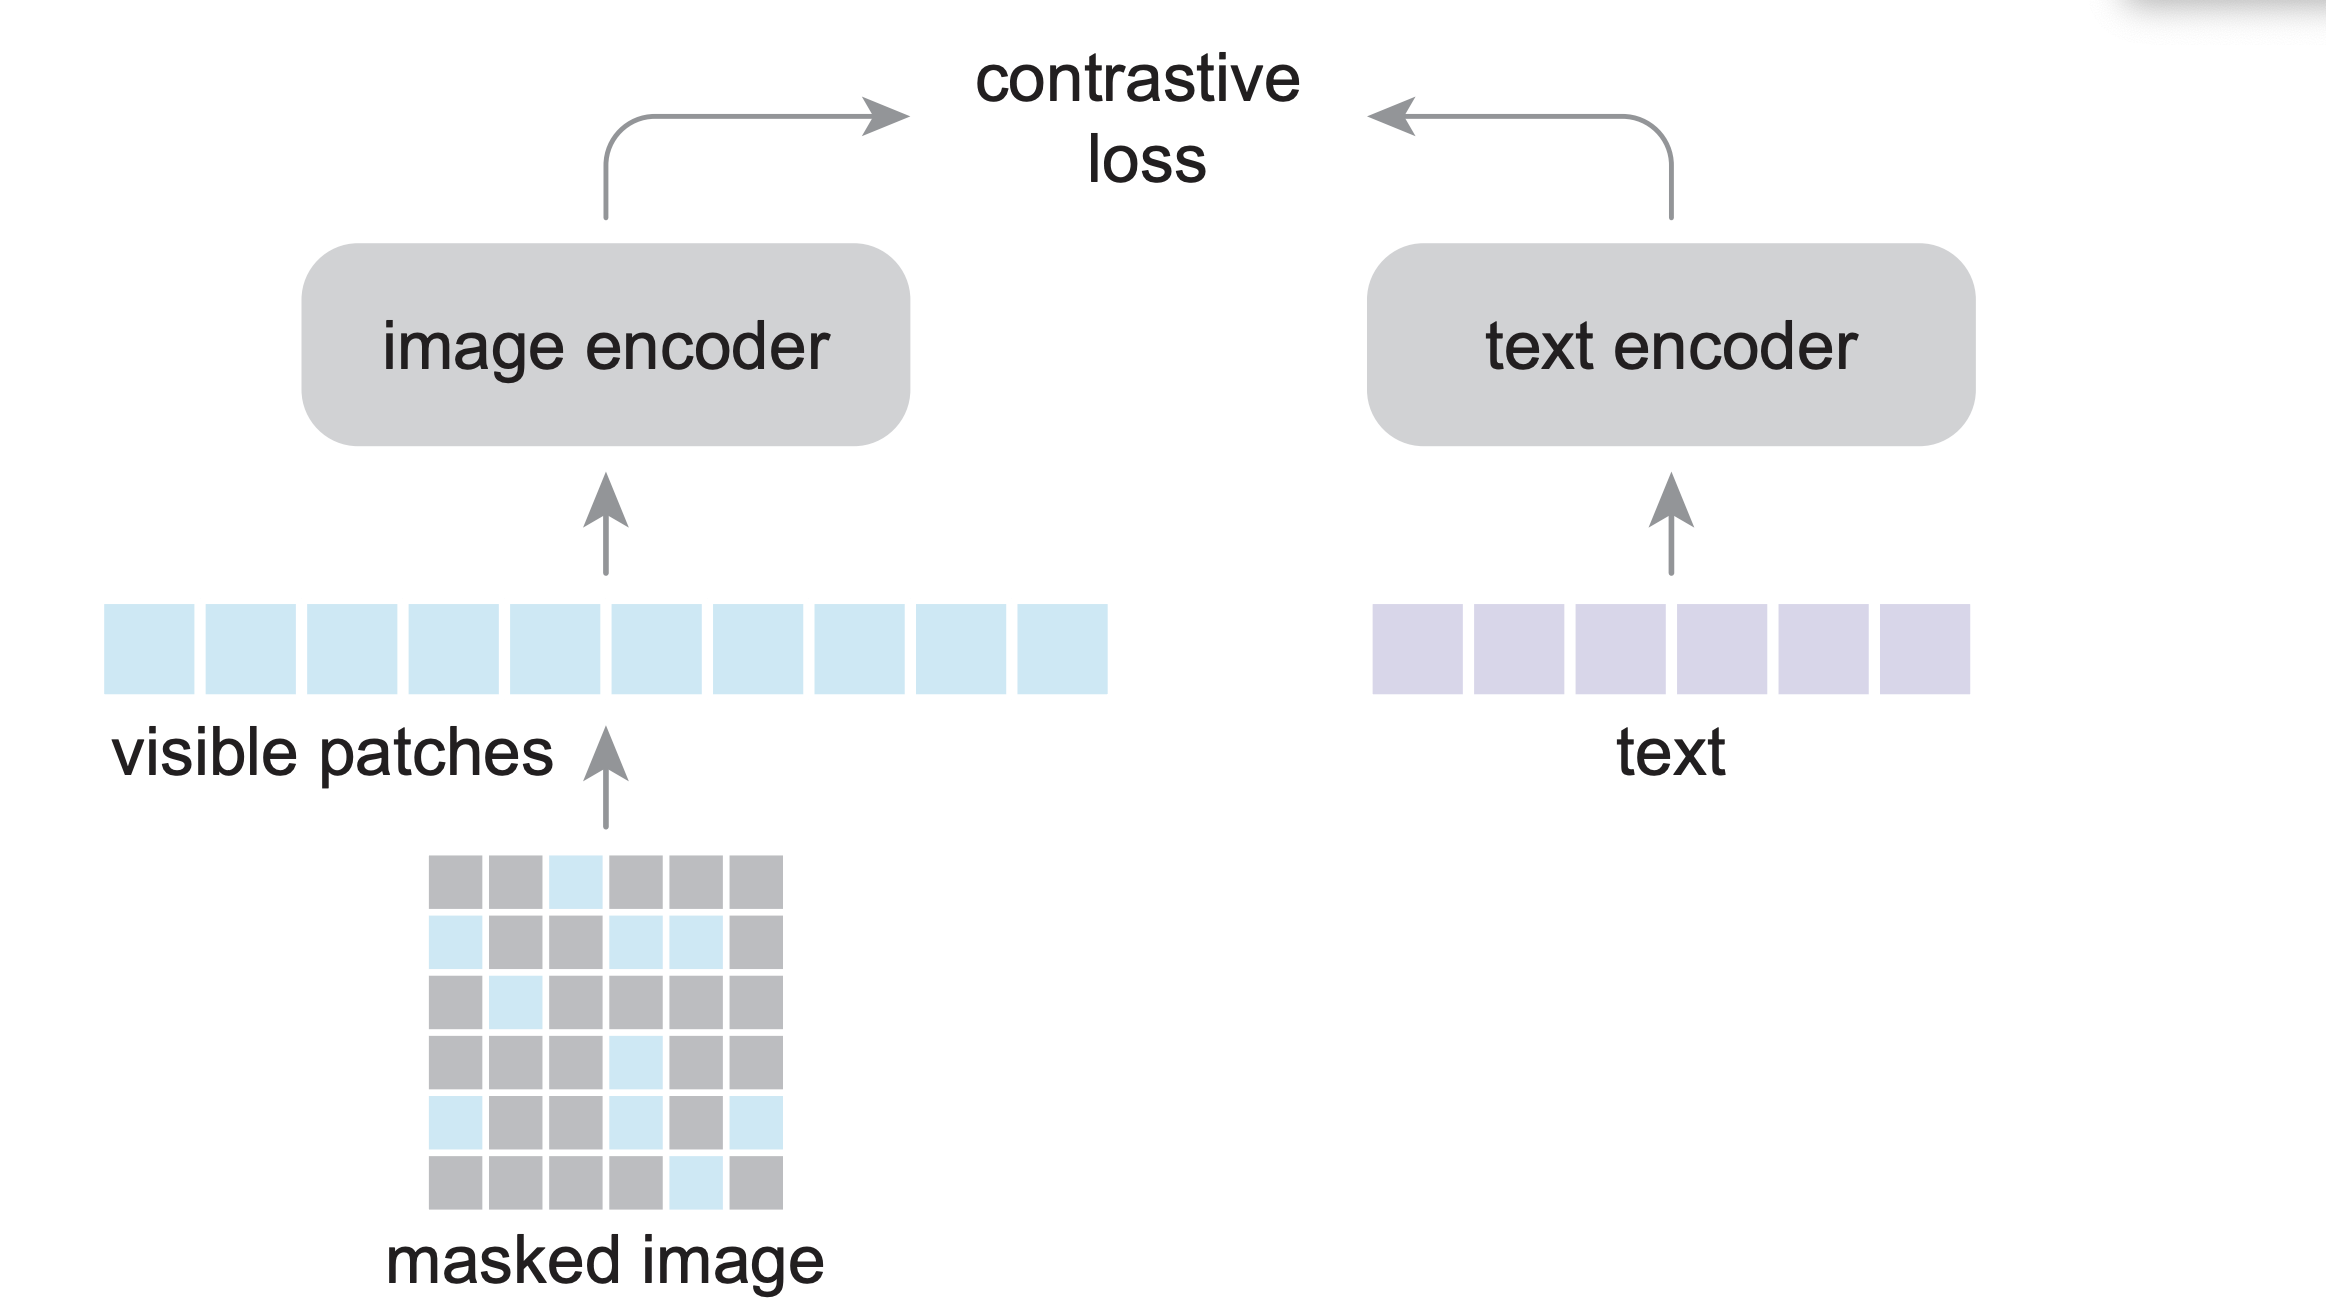
\includegraphics[width=13cm,height=8cm]{tikz/chapter11 - FLIP.png}};
\node[fill=white, xshift=-4.84cm, yshift=-0.6cm] {\large Visible Patches};
\node[fill=white, xshift=-3.1cm, yshift=-3.8cm] {\large Masked Image};
\node[fill=white, xshift=2.9cm, yshift=-0.6cm] {\large Text};
\node[fill=white, xshift=-0.17cm, yshift=3.3cm, align=center] {\large Contrastive \\ \large Loss};
\node[fill=mygray, xshift=-3.1cm, yshift=1.85cm, align=center] {\large Image Encoder};
\node[fill=mygray, xshift=2.9cm, yshift=1.85cm, align=center] {\large Text Encoder};

\end{tikzpicture}

\end{document}